
 In the case of uniform point distributions, we could obtain precise estimates for the threshold $n^*$ and use it to 
 choose between the truncation and expansion algorithms to achieve optimal complexity. However, when the source and 
 target distributions are highly non-uniform, as is the case in most practical applications, it is not as
 straightforward. Note that the expansion algorithm is advantageous when there are many sources within a FGT box and
 the truncation algorithm is more suitable otherwise. Hence, to achieve optimal complexity in the non-uniform case, we 
 need a hybrid algorithm that uses the expansion algorithm in regions with a high density of points and the 
 truncation algorithm in other regions. We use an {\em octree} \cite{clr90} data structure to efficiently
 separate out regions with a dense point distribution from regions with a sparse point distribution and use
 it to appropriately choose between the truncation and expansion algorithm in each region. A similar idea was
 used in \cite{veerapaneni08}.  
 
{\em Primer on octrees.} An octree is a tree data structure that is used for spatial decomposition. Every
node of an octree has a maximum of eight children. An octant with no children is
called a ``{\em leaf}'' and an octant with one or more children is
called an ``{\em interior octant}''. The only octant with no parent is the
 ``{\em root}'' and all other octants have exactly one parent. The depth of an octant 
 from the root is referred to as its ``{\em level}''. We use a ``{\em linear}'' octree
representation (i.e., we exclude interior octants) using the ``{\em
Morton encoding}'' scheme \cite{morton66}. Any octant in the domain can be uniquely
identified by specifying one of its vertices, also known as its ``{\em
anchor}'', and its level in the tree. By convention, the anchor of an
octant is its front lower left corner. 

\subsection{Octree based FGT algorithm}
\label{sc:octreefgt}

 Given a point distribution, we construct a linear octree such that there are no more than $m$ points contained within each leaf; we
 use the algorithm described in \cite{octPaper08} to do this. Note that regions with sparse point distributions will contain 
 leaves that are large in size and regions with dense point distributions will contain leaves that are small in size. Just as in 
 the uniform case, we partition the domain into FGT boxes of size $h = \sqrt{\delta}$. We denote the size of leaf $\ell$ by $|\ell|$.
 We use a heuristic parameter, $c$, to mark leaves as either ``Expand'' or ``Direct'' as follows (Figure \ref{f:directExpand}):

{\tt
\begin{algorithmic}
\STATE
  \FOR {each leaf $\ell$}
      \IF {$|\ell| > c h$}
          \STATE Mark $\ell$ as ``Direct''. 
      \ELSE
          \STATE Mark $\ell$ as ``Expand''. 
      \ENDIF
  \ENDFOR
\STATE
\end{algorithmic}
}

\begin{figure}
\begin{center}
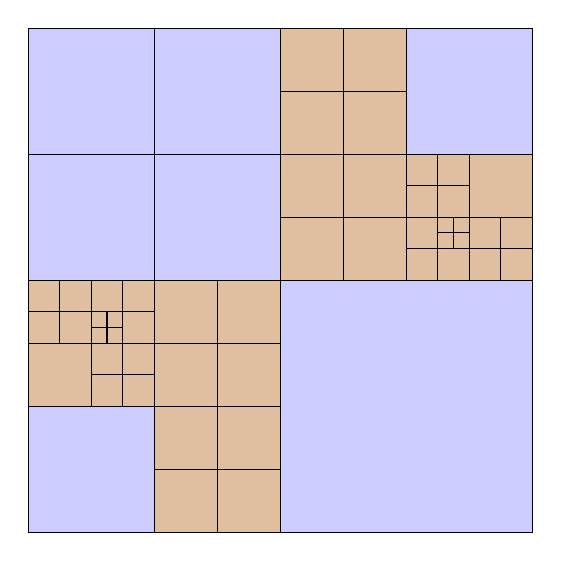
\begin{tikzpicture}[scale=0.4]

\draw[fill=blue!20] (0,8) rectangle +(8,8);
\draw[fill=blue!20] (8,0) rectangle +(8,8);
\draw[fill=blue!20] (0,0) rectangle +(4,4);
\draw[fill=blue!20] (12,12) rectangle +(4,4);

\draw[fill=brown!50] (4,0) rectangle +(4,4);
\draw[fill=brown!50] (0,4) rectangle +(4,4);
\draw[fill=brown!50] (4,4) rectangle +(4,4);
\draw[fill=brown!50] (8,8) rectangle +(4,4);
\draw[fill=brown!50] (8,12) rectangle +(4,4);
\draw[fill=brown!50] (12,8) rectangle +(4,4);

%Draw the initial octree
\draw[step = 8] (0,0) grid (16,16);
\draw[step = 4] (8,8) grid(16,16);
\draw[step = 4] (0,8) grid(8,16);
\draw[step = 2] (0,4) grid(4,8);
\draw[step = 2] (4,4) grid (8,8);
\draw[step = 2] (4,0) grid (8,4);
\draw[step = 1] (2,4) grid (4,8);    	
\draw[step = 1] (0,6) grid (2,8);
\draw[step = 0.5] (2,6) grid (3,7);

\draw[step = 2] (8,8) grid(12,16);
\draw[step = 2] (12,8) grid (16,12);
    	    	
\draw[step = 1] (12,8) grid (14,12);
\draw[step = 1] (14,8) grid (16,10);
\draw[step = 0.5] (13,9) grid (14,10);    	    	    	    	
    	    	    	    	
\end{tikzpicture}
\caption{\label{f:directExpand} The direct and expand leaves are colored in blue and brown, respectively.}  
\end{center}
\end{figure}

We denote the set of direct leaves by $T_d$ and use $T_e$ to represent the set of expand leaves. Next,
we describe the sequence of steps involved in this algorithm.

\begin{description}
\item[\textbf{S2W}] For each leaf $\ell \in T_e$ such that $|\ell| \leq h$, add the contributions from all sources within $\ell$
to the plane-wave expansion for the FGT box, $B$, that contains $\ell$ using (\ref{eqn:s2w}). For each leaf $\ell \in T_e$ such that $|\ell| > h$,
visit each FGT box $B$ that is contained within $\ell$ and form the plane-wave expansion for $B$ using the sources that are contained within $B$
as shown in (\ref{eqn:s2w}).

\item[\textbf{W2D}] Initialize the transform at all targets within some direct leaf to zero. For
 each target, $x$, within some direct leaf, find all FGT boxes, $B$, such that $\mathcal{I}[B]$ contains $x$ and
 add the contributions from the respective plane-wave expansion, $w_k$ to the transform at the target as: 

\beq F(x) \, +=\, \sum_{|k| \leq p} \hat{G}(k)  w_k e^{i \lambda k \cdot (x - c^B)} \label{eqn:w2d} \eeq

Note, that for any FGT box, $B$, which is contained within some direct leaf the corresponding $w_k$ is zero.

\item[\textbf{D2D}] For each source $y \in T_d$, find all targets $x \in T_d$ such that $x \in \mathcal{I}[y]$ and
 modify the transform at $x$ as:
  
\beq F(x) \,+=\, G_\delta(\norm{x - y}) f(y) \label{eqn:d2d} \eeq

\item[\textbf{W2L}] This step is identical to the W2L step discussed in Sections \ref{sc:fgt} and \ref{sc:sweep}.

\item[\textbf{D2L}] For each source, $y$, within some direct leaf, find all FGT boxes, $D$, such that $\mathcal{I}[y]$ intersects $D$ and
modify the local expansion, $v_k$, of $D$ as: 

\beq v_k  \,+=\, \, f(y) e^{i \lambda k \cdot (c^D - y)} \label{eqn:d2l} \eeq

\item[\textbf{L2T}] For each target, $x$, within some expand leaf, evaluate the transform using the local 
expansion of the FGT box, $D$, that contains $x$ using (\ref{eqn:l2t}).

\end{description}


\subsection{Parallel Implementation}
\label{sc:parallelnufgt}

Then the following are the different stages of the parallel algorithm:

{\em (i) S2W}. 

{\em (ii) S2W-Comm.} Because the boxes are partitioned by [RAHUL] and the octree is partitioned by Morton ordering, it is not necessary that the boxes contained in a leaf (or vice-versa) belong to the same processor. Therefore, after the S2W step, we send the plane-wave expansions formed in each processor to the owner of the respective boxes. Then, we visit each box $B \in T_e$ and add all the plane-wave expansions formed at different processors to obtain $\{w_k \}_{|k| \leq p}$.  

{\em (iii) W2D.} At this stage, all processors have finished forming the plane-wave expansions at their respective boxes. 
Now, we use this information to evaluate the influence of $T_e$ on $T_d$. Each box $B \in T_e$ must visit every target point $x \in T_d$ in its interaction list and evaluate the Gauss transform using
%
\beq F(x) = \sum_{|k| \leq p} e^{-\frac{\norm{z_k}^2}{4}} e^{i z_k \cdot (x - c^B)/\sqrt{\delta}} w_k \eeq
%
We perform a two-step communication to achieve this. In the first step, we send requests to the owners of boxes that are in the interaction lists of targets in $T_d$. In the second step, the owners send the plane-wave coefficients \footnote{ If $T_d$ receives any requests, it simply sends zero plane-wave coefficients. This can be avoided by an extra communication step}. 

{\em (iv) D2D.}
1. For each point (p) within each octant marked as Direct, compute the
point (A) in the -ve corner and the point (B) in the +ve corner of p's
interaction list. Note, the Morton ids of all points in the interaction
list of point p will be >= that of point A and <= that of point B.
2. Gather the Morton id of the first (in the Morton sorted list) direct
octant on each processor. This will give the smallest Morton id of
direct octants on each processor. Handle the case where some processors
do not contain any direct octants.
3. Figure out the processor with the greatest value <= A in the list
computed in step 2.
4. Figure out the processor with the greatest value <= B in the list
computed in step 2.
5. Send point p and the corresponding source f to all processors that
lie between the processors computed in step 3 and step 4. Note, we are 
using the property that if the Morton id of Octant C < Morton id of 
Octant D then the Morton id of any point within Octant C is >  Morton
id of Octant C and is < Morton id of Octant D.
6. For each point p recieved in step 5, compute the
point (A) in the -ve corner and the point (B) in the +ve corner of p's
interaction list. Find the direct octant O1 with the maximum Morton id that
is <= A and the direct octant O2 with the maximum Morton id that is <=
B. Loop over the set of Direct octants O with Morton ids >= that of O1
and <= that of O2. Loop over the set of points within O that lie in the
interaction list of p. For each of these points, add the contribution to
the Gauss transform from p.

{\em (v) W2L.} To allow execution of the sweeping algorithm independently on each processor, we exchange the plane-wave expansions of $\lfloor K/2 \rfloor ^3$ boundary boxes across adjacent processors. 


{\em (vi) D2L.} This step is a dual of the W2D. Here, we compute the influence of $T_d$ on $T_e$ by visiting every box $D \in T_e$ in the interaction list of a source $y \in T_d$ and modifying the local expansion as 
%
\beq v_k += \, f(y) e^{i z_k \cdot (c^D - y)/\sqrt{\delta}} \eeq
%
This requires a one-step communication: in each processor, we visit every source $y \in T_d$ 
and send its information ($y$ and $f(y)$) to processors that own boxes that are in $\mathcal{I}[y]$.

{\em (vii) L2T-Comm.} This step is a dual of S2W-Comm. Here, we send the local expansions formed at boxes in each processor 
to the processors that own leaf nodes that are contained within this FGT box. 


{\em (viii) L2T.} At this stage, all boxes must have formed their local expansions and $F(x)$ must have been computed at
 the points $x \in T_d$. The only remaining step is to compute $F(x)$ for points in $x \in T_e$ by using (\ref{eqn:l2t}) 
 which can be done independently in each processor. 

We summarize the overall algorithm and give the complexity estimates for the main steps in Algorithm \ref{a:ofgt}.  

\begin{algorithm}[!h]
\caption{ \label{a:ofgt}
\em Parallel FGT for non-uniform distributions}
{\tt
\begin{algorithmic}
\STATE Input: $N$ Points, $\delta$, $\epsilon$, $m$ and $c$
\STATE 1. Create a regular grid of FGT boxes partitioned across processors such that \\
 (A) the size of each box is $h = \sqrt{\delta}$, \\
 (B) each processor owns a sub-grid of boxes and \\
 (C) each box is owned by an unique processor. \\

\STATE 2. Construct a linear octree such that each leaf contains fewer than $m$ points. \\
\hfill $\bigO(\frac{N}{n_p} \log{\frac{N}{n_p}} + n_p \log{n_p})$

\STATE 3. Mark each leaf as either ``expand'' or ``direct'' based on $c$ and $\delta$.

\STATE 4. Partition the direct leaves across processors such that \\
  (A) they are globally sorted in the Morton ordering and \\
  (B) each leaf is owned by an unique processor.

\STATE 5. Partition the expand leaves across processors. 

\STATE 6. Execute S2W. \hfill $\bigO(p^3 \frac{N}{n_p})$

\STATE 7. Execute S2W-Comm. \hfill $\bigO(K^3 n_p)$

\STATE 8. Execute W2D. \hfill $\bigO(p^3 \frac{N}{n_p})$

\STATE 9. Execute D2D. \hfill $\bigO(p^3 \frac{N}{n_p})$

\STATE 10. Execute W2L. \\
 \hfill $\bigO(p^3 \frac{|B|}{n_p} + K (\frac{|B|}{n_p})^{\frac{2}{3}} + K^2(\frac{|B|}{n_p})^{\frac{1}{3}} + K^3 )$ 

\STATE 11. Execute D2L. \hfill $\bigO(p^3 \frac{N}{n_p})$

\STATE 12. Execute L2T-Comm. \hfill $\bigO(K^3 n_p)$

\STATE 13. Execute L2T. \hfill $\bigO( p^3\frac{N}{n_p})$
\end{algorithmic}
}
\end{algorithm}


